% This template written by Dr. Helmstutler.
% If your questions about this document cannot be answered by a lot of research, see Dr. H in Trinkle 128.
% Suggested reference:  "Math Into LaTeX" by George Gratzer.

\documentclass[11pt]{article}
\usepackage{amsmath, amsthm, amsfonts, amssymb, latexsym}
\usepackage{tensor} % For properly aligned mixed upper/lower indices
\usepackage[mathscr]{euscript} % For script font
\usepackage{graphicx}

% The following is just a suggestion.  Theoremstyle declarations left to discretion of student/advisor.

\newtheorem{thm}{Theorem}
\newtheorem{cor}[thm]{Corollary}
\newtheorem{lem}[thm]{Lemma}
\newtheorem{prop}[thm]{Proposition}
\newtheorem{claim}[thm]{Claim}
\newtheorem*{unno_claim}{Claim}

\theoremstyle{definition}
\newtheorem{defn}[thm]{Definition}
\newtheorem{ex}[thm]{Example}
\newtheorem*{quest}{Question}
\newtheorem*{unno_ass}{Assumption}
\newtheorem*{unno_notat}{Notation}

\theoremstyle{remark}
\newtheorem*{unno_rem}{Remark}
\newtheorem*{unno_note}{Note}

% For page width.  Do not disturb.
\oddsidemargin=0.0in \evensidemargin=0.0in \textwidth=6.5in

% For paper height.  Do not disturb.
\topmargin=-0.5in \textheight=9.0in

% For no paragraph indents.  Style choice left to student/advisor.
% \setlength{\parindent}{0pt}

% Various commands.
\newcommand{\scr}[1]{\mathscr{#1}}
\newcommand{\sU}{\scr{U}}
\newcommand{\sV}{\scr{V}}

\newcommand{\bX}{\mathbf{X}}
\newcommand{\bx}{\mathbf{x}}
\newcommand{\bY}{\mathbf{Y}}
\newcommand{\by}{\mathbf{y}}
\newcommand{\bT}{\mathbf{T}}
\newcommand{\bS}{\mathbf{S}}
\newcommand{\bn}{\mathbf{n}}
\newcommand{\bN}{\mathbf{N}}
\newcommand{\bg}{\boldsymbol{\gamma}}
\newcommand{\ba}{\boldsymbol{\alpha}}
\newcommand{\zero}{\mathbf{0}}
% TODO: Weingarten Map L
\newcommand{\wg}{L}
\newcommand{\RR}{\mathbb{R}}
\newcommand{\ptl}{\partial}
\newcommand{\Ck}{C^k}
\newcommand{\eps}{\varepsilon}
\newcommand{\inv}{^{-1}}
\newcommand{\ra}{\rangle}
\newcommand{\la}{\langle}
\newcommand{\Cfl}{\tensor{\Gamma}{_{ij}^k}}
\newcommand{\del}{\partial}
\renewcommand{\Re}{\text{Re}}
\renewcommand{\Im}{\text{Im}}

\newcommand{\buildset}[2]{\left\{#1\;\middle\vert\;#2\right\}}

\graphicspath{ {/figures/} }
\begin{document}

%%%%%%%%%%%%%%%%
%% Title Page %%
%%%%%%%%%%%%%%%%

% Do not disturb the spacing parameters.

\protect{\thispagestyle{empty}}

\begin{center}

\LARGE

\phantom{1}

\vspace{1.5in}

\sc Surface Theory, Miminal Surfaces, and Weierstrass Representation \normalfont

\Large

\vspace{1.0in}

Christopher A.\ Hunt

\vfill

submitted in partial fulfillment of the requirements for Honors in Mathematics at the
University of Mary Washington

\vspace{0.5in}

Fredericksburg, Virginia

\vspace{0.5in}

April 2014

\normalsize

\vspace{1.0in}

\end{center}

\pagebreak

%%%%%%%%%%%%%%%%%%%%
%% Signature Page %%
%%%%%%%%%%%%%%%%%%%%

% Do not disturb the spacing parameters.

\protect{\thispagestyle{empty}}

\phantom{1}

\vspace{0.5in}

\noindent  This thesis by \textbf{John Q.\ Student} is accepted in its present form as satisfying the thesis requirement
for Honors in Mathematics.

\vspace{1.0in}

% Thesis advisor FIRST, then readers alphabetically.

\begin{tabular}{p{1.0in}l}
\sc Date & \sc Approved \\[.65in]
\rule{0.85in}{0.5pt} & \rule{2.6in}{0.5pt}\\
& Yuan-Jen\ Chiang, Ph.D.\\    % Advisor
& thesis advisor\\[.65in]
\rule{0.85in}{0.5pt} & \rule{2.6in}{0.5pt}\\
& Randall D.\ Helmstutler, Ph.D.\\  % Reader #1
& committee member\\[.65in]
\rule{0.85in}{0.5pt} & \rule{2.6in}{0.5pt}\\
& Jangwoon\ Lee, Ph.D.\\   % Reader #2
& committee member
\end{tabular}

\pagebreak

%%%%%%%%%%%%%%
%% Contents %%
%%%%%%%%%%%%%%

% This creates the table of contents, but does not paginate it.  Do not disturb.

\phantom{1}

\vspace{0.5in}

\tableofcontents{\protect\thispagestyle{empty}}

\pagebreak

\setcounter{page}{1}

%%%%%%%%%%%%%%
%% Abstract %%
%%%%%%%%%%%%%%

\begin{abstract}
\noindent  Here's what we're going to do.
\end{abstract}

\vspace{0.25in}

%%%%%%%%%%%%%%%%%%%%%%
%% Exposition Below %%
%%%%%%%%%%%%%%%%%%%%%%

{%!TEX root=thesis.tex
\section{Surface Theory}

Investigating the properties of surfaces will form the basis on which our journey towards minimal surfaces rests. We will brave the perils that come in defining surfaces, and then use calculus on these surfaces to approximate the behavior at a point and extract information about the surface by extending on that approximation. Along the way we will make and derive various tools used for analyzing these surfaces, some of which we will bring along with us to Minimal Surfaces, others are interesting nonetheless and help to illustrate some of the connections between Differential Geometry and various other branches of mathematics. In this chapter, we will also look at parallels between these surfaces in $\RR^3$ and higher dimensional Riemannian manifolds, though only briefly. In general our reference for this section will be~\cite{MP77} which, while not as recent as some other texts, gives a very clean, if compact, view of the subject.

\subsection{Defining Surfaces in $\RR^3$}

% Simple surface
% TODO: Check to see if U needs to be connected - insert mention of being path-connected per Oprea p69
% Refactored
Defining surfaces is not particularly difficult, but our methods require a set of considerations that can be subtle. We will first define a \emph{simple surface}, or coordinate patch, which represents a small open section of a larger surface. After considering that, we define a \emph{coordinate transformation}, a type of function whose presence between these patches implies some geometry-preserving properties. That done, we finally build up surfaces using an open covering of these coordinate patches, with the requirement that a coordinate transformation exist on their intersection. Along the way we will have plenty of examples to illustrate specific techniques and concepts introduced.

\begin{defn} % def: Simple Surface
  Let $\sU$ be an open subset of $\RR^2$, then a $C^k$ function $\bx: \sU \to \RR^3$, with $(k \ge 1)$ written $\bx(u_1, u_2)$, is known as a \emph{simple surface} if it is injective and regular. The condition for regularity is that
  \[
    \frac{\partial\bx}{\partial u_1} \times \frac{\partial\bx}{\partial u_2} \neq \zero
  \]
  across the domain of $\bx$. The function $\bx$ may also be referred to as a \emph{coordinate patch}.
\end{defn}

This definition is exactly what we want. Conceptually, the regularity of $\bx$ ensures that the mapping of $\sU$ to $\RR^3$ doesn't create any sharp creases or corners, but perhaps more relevant to our purposes, it also ensures that the partial derivatives form a linearly independent set. This will be critical later on.

% TODO: Refactor and incorporate smooth/one-to-one
\begin{ex} % ex: Monge Patch example
  Before going any further we introduce the \emph{monge patch}, a simple surface that will be instrumental as a simple example on which we can carry out our calculations. Let $f(x, y) = z$ be a function, then we can use this in the parameterization of our patch as follows: $\bx(u, v) = (u, v, f(u, v))$. Notice that
  \begin{align*}
    \frac{\partial\bx}{\partial u} \times \frac{\partial\bx}{\partial v} &= \left(-\frac{\partial f}{\partial u}, -\frac{\partial f}{\partial v}, 1\right)\\
    &\neq \zero
  \end{align*}
  so it really is a simple surface.
\end{ex}

\begin{ex} % ex: Surface of revolution
  \label{ex:revolution}
  % TODO: Fix akward wording.
  Another fine example is the \emph{surface of revolution}. Given a curve in the $(r, z)$ with $r = r(t) > 0$ and $z = z(t)$, the surface of revolution generated by this curve (via rotation about the z-axis, is given by
  \[
    \bx(t, \theta) = (r(t)\cos\theta, r(t)\sin\theta, z(t)) \ .
  \]

  % NOTE: p15
  Assuming the curve is regular and injective, we can show that a surface of revolution really is a simple surface by checking. (A curve, say $\ba : (a, b) \to \RR^3$ is considered \emph{regular} when $\frac{d\ba}{dt} \neq 0$ for any $t$ in $(a, b)$.)

  A quick calculation yields the following:
  \begin{align*}
    \bx_1 &= (\dot{r}\cos{\theta}, \dot{r}\sin{\theta}, \dot{z})\\
    \bx_2 &= (-r(t)\sin{\theta}, r(t)\cos{\theta}, 0)\\
    \bx_1 \times \bx_2 &= (-\dot{z} r(t) \cos{\theta}, -\dot{z} r(t) \sin{\theta}, \dot{r}r(t)) \ ,
  \end{align*}
  which is not $\zero$ since $r(t) > 0$, and then the original curve was regular so $\dot{r}, \dot{z} \neq 0$.
\end{ex}
% TODO: Example of an irregular surface

% TODO: Refactor
\begin{defn} % def: Coordinate transformation definition (LOC: p79)
  Let $\sU, \sV$ be open subsets of $\RR^2$. A $C^k$ \emph{coordinate transformation} is an injective $C^k$ function $f: \sV \to \sU$ whose inverse $g:\sU \to \sV$ is also of class $C^k$. 
\end{defn}


As we continue we will lean heavily on the structure-preserving properties of these coordinate transformations, so we will take some time with them now to fully appreciate their impact. The following result we will need shortly. Let $f$ be a function from $\RR^2$ to itself and recall the \emph{Jacobian} of $f$ is the matrix-valued function of partial derivatives, denoted $J(f)$ given by
\begingroup
  \renewcommand*{\arraystretch}{1.4}
  \begin{align*}
    J(f) &= \left(
    \begin{array}{cc}
      \frac{\del f_1}{\del x_1} & \frac{\del f_1}{\del x_2}\\
      \frac{\del f_2}{\del x_1} & \frac{\del f_2}{\del x_2}
    \end{array}
    \right) \ .
  \end{align*}
\endgroup

\begin{lem}
  Let $f:\sV \to \sU$ be a coordinate transformation, then $J(f)$ is nonsingular.
\end{lem}

\begin{proof}
  We can write $f(v^1, v^2) = (f^1(v^1, v^2), f^2(v^1, v^2))$ where each $f^i$ is the $i$-th parameter function for $f$. Then since $f$ is a coordinate transformation there is an inverse function $g$ which can be written similar to $f$ as $g(u^1, u^2) = (g^1(u^1, u^2), g^2(u^1, u^2))$. Then since $f$ and $g$ are inverses we have
  \begin{align*}
    f^1(g^1, g^2) &= u^1\\
    f^2(g^1, g^2) &= u^2 \ .
  \end{align*}
  % TODO: Fix wording.
  Herein we will be Taking the partial derivative of each on $u^1$ and $u^2$ yields
  \newcommand{\fdg}[3]{\frac{\del f^{#1}}{\del v^{#2}} \cdot \frac{\del g^{#2}}{\del u^{#3}}}
  \begin{equation*}
    \begin{aligned}[c]
      \fdg{1}{1}{1} + \fdg{1}{2}{1} &= 1\\
      \fdg{2}{1}{1} + \fdg{1}{2}{1} &= 0
    \end{aligned}\qquad
    \begin{aligned}[c]
      \fdg{1}{1}{2} + \fdg{1}{2}{2} &= 0\\
      \fdg{2}{1}{2} + \fdg{2}{2}{2} &= 1 \ ,
    \end{aligned}
  \end{equation*}
  which is certainly nonsingular. Then since $f$ was generic, coordinate transformations have nonsingular Jacobian.
\end{proof}

% TODO: Expand on the below
\begin{lem}
  % TODO: Fix wording.
  Something about having the same image as $\bx$.
\end{lem}

\newcommand{\xdf}[2]{\frac{\del\bx}{\del u^{#1}}\cdot\frac{\del f^{#1}}{\del v^{#2}}}
\newcommand{\df}[2]{\frac{\del f^{#1}}{\del v^{#2}}}
\newcommand{\dx}[1]{\frac{\del\bx}{\del u^{#1}}}
\begin{proof}
  Since
  \begin{gather*}
    \left(\xdf{1}{1} + \xdf{2}{1}\right) \times \left(\xdf{1}{2} + \xdf{2}{2}\right)\\
    \left(\left(\xdf{1}{1} + \xdf{2}{1}\right) \times \xdf{1}{2}\right) + \left(\left(\xdf{1}{1} + \xdf{2}{1}\right) \times \xdf{2}{2}\right)\\
    \left(\xdf{1}{1} \times \xdf{1}{2}\right) + \left(\xdf{2}{1} \times \xdf{1}{2}\right) + \left(\xdf{1}{1} \times \xdf{2}{2}\right) + \left(\xdf{2}{1} \times \xdf{2}{2}\right)\\
    0 + \left(\xdf{2}{1} \times \xdf{1}{2}\right) + \left(\xdf{1}{1} \times \xdf{2}{2}\right) + 0\\
    \df{2}{1}\cdot\df{1}{2}\left(\dx{2} \times \dx{1}\right) + \df{1}{1}\cdot\df{2}{2}\left(\dx{1} \times \dx{2}\right)\\
    \df{2}{1}\cdot\df{1}{2}\left(-\dx{1} \times \dx{2}\right) + \df{1}{1}\cdot\df{2}{2}\left(\dx{1} \times \dx{2}\right)\\
    \left(\df{1}{1}\cdot\df{2}{2} - \df{2}{1}\cdot\df{1}{2}\right)\left(\dx{1} \times \dx{2}\right)\\
    \text{det}(J(f))\left(\dx{1} \times \dx{2}\right)
  \end{gather*}
  then since $J(f)$ is nonzero
\end{proof}

In the propositions that follow we will see that the coordinate transformation preserves geometric properties regardless of parameterization. 

% TODO: Coordinate transformation information

Before getting to surfaces, we need to put an additional restriction on the coordinate patches that we build them with.

Consider the inverse function for a coordinate patch $\bx$ from some subset $M$ of $\RR^3$ back to $\sU$, $\bx^{-1}: M \to \RR^2$ for some subset $M$ of $\RR^3$. We will say that this function is \emph{continuous} at a point $p$ if there is a neighborhood $U_p$ around the point such that $\bx^{-1}(U_P)\subset \sU$. The patch $\bx$ is considered \emph{proper} if $\bx^{-1}$ is continuous for all $P \in \bx(\sU)$.

\begin{defn} % def: Surface (LOC: p89)
  A $C^k$ \emph{surface} in $\RR^3$ is a subset $M \subset \RR^3$ such that for every point $p \in M$ there is a proper $C^k$ coordinate patch whose image is in $M$ and which contains an $\eps$-neighborhood of $p$ for some $\eps > 0$. Furthermore, if both $\bx: \sU \to \RR^3$ and $\by: \sV \to \RR^3$ are such coordinate patches with $\sU^\prime = \bx(\sU), \sV^\prime = \by(\sV)$, then $y^{-1} \circ \bx: (x^{-1}(\sU^\prime \cap \sV^\prime)) \to (y^{-1}(\sU^\prime \cap \sV^\prime))$ is a $C^k$ coordinate transformation.
\end{defn}

As stated previously, the cooridnate transformation has a preserving property but that isn't the whole story. It is really the case that we define a property \emph{as} geometric when we can show that it is preserved under coordinate transformation. This will ensure that the property exists for a surface regardless of parameterization which is important here since it is very likely that multiple such parameterizations exist.

% TODO: Picture of the coordinate transformation requirement.

% TODO: Explanation of the coordinate transformation requirement.

% TODO: Example of a reason why this is necessary.

% TODO: Finish example of definition of the coordinate patches for a torus.
One surface of revolution, the torus, has a patch given by the parameterization
\[
  \bx(u, v) = ((2 + \cos u)\cos v, (2 + \cos u) \sin v, \sin u)
\]
with the domain $\sU = \buildset{(u, v) \in \RR^2}{-\pi < u, v < \pi}$.

If we look at the diagram below we can see the areas not covered by this coordinate patch highlighted.
\begin{figure*}[t] % fig: Torus
  \centering
  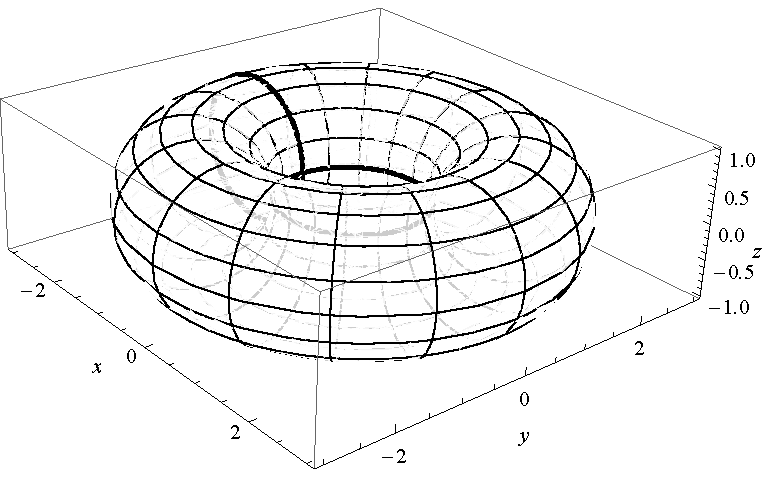
\includegraphics[width=0.5\textwidth]{figures/torus.pdf}
  \caption{Test}
\end{figure*}
In this case finding additional patches so the surface is covered is not difficult. We can use the same parameterization but with different bounds on the domain. If we let
\begin{align*}
  \sU_1 &= \buildset{(u, v) \in \RR^2}{-\pi < u < \pi, \frac{3\pi}{4} < v < \frac{5\pi}{4}}\\
  \sU_2 &= \buildset{(u, v) \in \RR^2}{\frac{5\pi}{6} < u < \frac{7\pi}{6}, \frac{\pi}{4} < v < \frac{7\pi}{4}}\\
  \sU_3 &= \buildset{(u, v) \in \RR^2}{\frac{5\pi}{6} < u < \frac{7\pi}{6}, -\frac{3\pi}{4} < v < \frac{3\pi}{4}}
\end{align*}
with the same parameterization for each, these will cover the outside of the torus on the negative $x$ side, the inside of the torus on the negative $x$ side, and the inside of the torus on the positive $x$ side, respectively.

% TODO: Check one of the intersections as a coordinate transformation


%%%%%%%%%%%%%%%%%%%%%%%%
%                      %
% CALCULUS ON SURFACES %
%                      %
%%%%%%%%%%%%%%%%%%%%%%%%

\subsection{Calculus on Surfaces}

% TODO: Explanation of title and the concepts that we will be introducing
This portion of our exploration we will define a structure, the $tangent plane$, on the surfaces introduced above. We will also show that tangent planes remain preserved under reparameterization on a surface constructed with the coordinate transformation requirement we have imposed. The tangent plane will give us a linear approximation of the behavior of the surface at a specific point on which we will build our tools in the next section, and the fact that it is preserved under coordinate transformation will obviate the need to check each tensor individually.

\begin{defn} % def: Tangent vector.
  We consider two specific tangent vectors on a surface, the 
\end{defn}

\begin{unno_rem}
  We typically consider the partial derivative as the tangent vector of a curve holding one parameter of the function constant, so planting the base of the vector at the point at which it is evaluated.
\end{unno_rem}

% Continuity

% Properness

\begin{defn}
  The \emph{tangent plane} to a simple surface  $\bx: \sU \to \RR^3$ at the point $p = \bx(a, b)$ is the plane through $p$ perpendicular to $\bx_1(a, b) \times \bx_2(a, b)$. The \emph{unit normal} to the surface at $p$ is $\bn(a, b) = \frac{\bx_1 \times \bx_2}{\left|\bx_1 \times \bx_2\right|}$, where the right-hand side is evaluated at $(a, b)$. Note that $\bn(a, b)$ exists because $\bx_1 \times \bx_2 \neq 0$. It is perpendicular to the tangent plane at $p$.
\end{defn}

\begin{unno_rem}
  There are a few things to notice here. First, as $\bx_1$ and $\bx_2$ form a basis for the tangent plane and the unit normal is perpendicular to both, all together these three vectors form a basis for $\RR^3$. This will be useful later on as we consider the second derivative of curves at a point and will calculate them to put it into the context of the tangent plane.
\end{unno_rem}

% TODO: Theorem of tangent plane preservation under coordinate transformation

\subsection{Tensors and Operators on Surfaces}

In this section we discover some of the tools that we will use to figure out the properties of surfaces in the next. Notice as we travel that the majority of these forms and tensors are really capturing very simple information, but we turn around and use them in combination to represent more complex or subtle properties of the surface. For this section assume that our operations are taking place on a simple surface and, as the tangent plane being \emph{geometric} (i.e. independent of parameterization) was shown in the last section, take these objects built upon it to inherit the same property.

% First fundamental form and metric tensor
\begin{unno_rem}
  One of the most fundamental operations in Euclidean space, allowing us notions of distance and angles between vectors, is the dot product (or more generally, the \emph{inner product}). We wish to have the same capability on our surface. To motivate our construction, consider a surface $M \subset \RR^3$, $P$ a point on the surface, and two vectors $\bX$ and $\bY$ tangent to $M$ at $P$. Since $\bx_1$, $\bx_2$ form a basis for the tangent plane, in which $\bX$ and $\bY$ lie, we can write them as a linear combination and further, compute their inner product (denoted henceforth as $\la\phantom{x},\phantom{x}\ra$)
  \begin{align*}
    \bX &= \sum X^i\bx_i\\
    \bY &= \sum Y^j\bx_j\\
    \la\bX, \bY\ra &= \sum X^iY^j\la\bx_i, \bx_j\ra \ .
  \end{align*}
  With this in mind we make the following definition.
\end{unno_rem}

\begin{defn}
  The \emph{metric coefficients} are the functions defined by
  \[
    g_{ij}(u, v) = \la\bx_i(u, v), \bx_j(u, v)\ra \text{ or } g_{ij} = \la\bx_i, \bx_j\ra \ .
  \]
   % TODO: Expand here.
\end{defn}

% TODO: Properties of g_{ij}

% TODO: Finish g_{ij} computation example using surface of revolution
\begin{ex}
  Using our definition above, let's find the metric coefficients for a surface of revolution. Recall the parameterization and first partial derivatives found in example~\ref{ex:revolution},
  \begin{align*}
    \bx_1 &= (\dot{r}\cos{\theta}, \dot{r}\sin{\theta}, \dot{z})\\
    \bx_2 &= (-r(t)\sin{\theta}, r(t)\cos{\theta}, 0) \ .
  \end{align*}
  Then calculating the relevant inner products yields
  \[
    g_{ij} = \left(\begin{array}{cc}
      \dot{r}^2 + \dot{z}^2 & 0\\
      0 & \dot{r}^2
    \end{array}\right)
  \]
\end{ex}

% Second fundamental form
We make two notational additions: $\bx_{ij} = \frac{\partial^2\bx}{\partial u^j \partial u^i}$ and $\bS = \bn \times \bT$, $\bS$ is the \emph{intrinsic normal} of a curve $\gamma$. p103. Then it makes sense when we consider $\kappa_n(s) = \left\la\bg^{\prime\prime}(s), \bn(\gamma^1(s), \gamma^2(s))\right\ra$ since this will show any change between how the surface represented by the curve is tending to change and how it currently is (i.e. how the surface in which the curve is is curving through space). Also consider $\kappa_g(s) = \left\la\bg^{\prime\prime}, \bS(s)\right\ra$, then this is going to show how the curve is curving in the surface since $\bS$ is going to accomodate any changes resulting from a previous change and any changes resulting from a curvature of the surface itself.

$\kappa(s)\bN(s) = \bT^\prime(s) = \bg^{\prime\prime}(s) = \kappa_n(s)\bn + \kappa_g(s)\bS(s)$

% TODO: Refactor
Definition (103): The \emph{normal curvature} of a unit speed curve $\bg$ is the normal component of $\bg^{\prime\prime}$ (i.e. is $\kappa_n$). The \emph{geodesic curvature} of $\bg$ is the component of $\bg^{\prime\prime}$ in the direction of $\bS = \bn \times \bT$ (i.e. is $\kappa_g$).

So then this $\bN$ is a linear combination of the other two.

The \emph{coefficients of the second fundamental form} of a simple surface $\bx: \sU \to \RR^3$ are the functions $L_{ij}$ defined on $\sU$ by $L_{ij} = \left\la\bx_{ij}, \bn\right\ra$. This measures the normal component of $\bx_{ij}$.

Comment: What does the second derivative look like, and what does it give us.

The christoffel symbols are the functions $\Cfl (1 \le i, j, k \le 2)$ defined on $\sU$ by $\Cfl = \sum\limits_{l = 1}^2 \left\la \bx_{ij}, \bx_{l}\right\ra g^{lk}$. This measures the tangential components of $\bx_{ij}$.

Emphasis on thinking about these forms as assigning values to any two vectors. This is the second fundamental form because it is a symmetric bilinear form on $T_P M$

% Christoffel symbols

% Weingarten Map

\subsection{Curvature}

We considered surface patches, surfaces as being composed of these patches and that with the requirement of a coordinate transformation existing in-between each surface patch making up a surface we preserve geometric properties (with one exception or two like the sign of the normal which we will just say that our surface is orientable that way we don't have to worry about it). 

Next we consider concepts of curvature. As we consider a curve in the surface that curve has a unique parameterization in terms of the surface patch in which it is residing. We can write it as $\bg(t) = x(\bg^1(t), \bg^2(t))$. Then we consider the way in which the curve curves through the surface, and that takes two forms, normal and geodesic curvature. We will show that normal curvature approximates the change of the surface itself while geodesic curvature approximates the change of the curve's trajectory within the surface. 

The first derivative of a curve at a point gives us that curve's trajectory, and since we're interested in the change in this trajectory we're interested in the second derivative here which can be represented using the basis we described in the previous section. Recall the tangent plane introduced previously, we have seen that at any point we can use the first partial derivatives as a basis for this tangent plane. Then along with the normal to this plane we have a basis for $\RR^3$. Some of the symbols we're going to introduce tie in here as they are the coefficients of these basis vectors for the second derivative of a curve at a point.

All we're doing here is finding two vectors ($\bT$ and $\bS$) that are tied to the curve and 

\begin{defn} % def: Normal and geodesic curvature
  The \emph{normal curvature}

\end{defn}

% Normal Curvature

% Geodesic curvature

% Geodesics
Geodesics have some fun properties, one of which is that the shortest distance between two points in a (connected, complete?) surface will be a geodesic (notice that the converse is not true, counterexample using a sphere where two points will have a great circle that goes between then and only one of the curves that make up this circle ).

% Parallel translate
The difficulty with parallel translation is when you're not sure what part you aren't understanding. Is transport the opaque word that needs clarification or is it information? Depending on your background the specific wording may not give sufficient context for understanding what to expect when considering the subject. The part of transport to consider here is the idea of `preservation', when transporting something you have a set of things that you want to preserve (within reasonable bounds) and something that you want to change (in most cases this is reserved for simply the location being changes). In this case what we want to preserve is the orientation of a vector in relation to the surface, and so when we parallel translate a vector along a curve what we're doing is coming up with a method for, at each point on the curve, concerning ourselves with a vector that, from within the surface itself, would look identical as it points off of the surface.

% Principle Curvatures

% ex: #8.5 on page 137 calculating on surface of revolution or 8.10, or both.
% Mean Curvature

% Gaussian Curvature

% Gauss Map

\subsection{Manifolds}}
\pagebreak
{%!TEX root=thesis.tex
\section{Minimal Surfaces}

Minimal surfaces are found at the intersection of a number of different areas in mathematics. A side-effect of this is a great number of characterizations for the definition of a minimal surface. We will first define minimal surfaces using the language of surface theory that we developed in the previous chapter, then we will continue in that same vein to view various properties of minimal surfaces using the tensors and concepts developed previously. Having done that we will take a slightly different approach to build up minimal surfaces, as surfaces of least area, which will shape and prepare us for the discussion of the next chapter.

\subsection{Minimal Surfaces in the Language of Surface Theory}

  Minimal surfaces are surfaces with mean curvature everywhere equal to zero. Without an intuitive idea about mean curvature and the implications this seems a dry, technical statement, but the reality couldn't be further from the truth. Recall the calculation of mean curvature from the previous chapter, Equation~\ref{eq:mean_curvature}. We have something of a geometric intuition built up around this definition, but the difficulty in its calculation lies with the incorporation of the Weingarten Map. With this as the medium we must travel through each time, calculation becomes cumbersome. We will show in the rest of this chapter a somewhat easier method of approaching surfaces that will lend itself well to calculation.  

\subsection{Properties of Minimal Surfaces}
  There are several properties of minimal surfaces that we'd like to highlight here.

  \begin{thm}
    If a surface of revolution $M$ is minimal, then $M$ is contained in either a plane or catenoid.
  \end{thm}
  \begin{proof}
    See~\cite{Opr07} Theorem 3.5.7.
  \end{proof}

  We make the next definition to highlight an interesting fact about minimal surfaces.
  \begin{defn}
    We call a surface \emph{ruled} if, given two curves $\alpha$ and $\beta$, we can find a parameterization for the surface of the form
    \[
      \bx(s, t) = \alpha(s) + t\beta(s).
    \]
    In terms of the construction of the surface we can think of this as if we travel along $\alpha$ and at each point the surface is the sheet formed between $\alpha$ and $\beta$ mediated by the second parameter $t$. 
  \end{defn}

  \begin{thm}
    Any ruled minimal surface in $\RR^3$ is part of a plane or a helicoid.
  \end{thm}
  \begin{proof}
    See~\cite{Opr07} Theorem 4.2.6.
  \end{proof}

  This next one is less of a property and more of an example, in part to motivate the discussion of the next chapter.

  \begin{ex}
    \label{ex:ennepers_surface}
    Let $M$ be the surface parameterized by the patch $\bx(u, v) = \left(u - \frac{u^3}{3} + uv^2, v - \frac{v^3}{3} + vu^2, u^2 - v^2\right)$. This is known as \emph{Enneper's Surface}. We can see one view of it in Figure~\ref{fig:ennepers_surface}.

    \begin{figure}[t] % fig: Torus
      \centering
      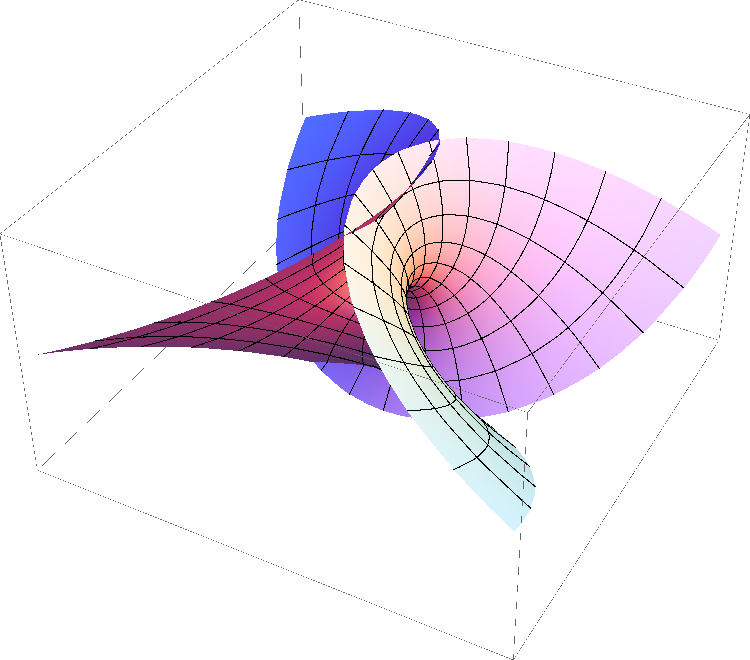
\includegraphics[width=0.5\textwidth]{figures/ennepers_surface.pdf}
      \caption{Enneper's Surface.}
      \label{fig:ennepers_surface}
    \end{figure}
  \end{ex}

\subsection{A Different Approach to Minimal Surfaces}
  \label{ss:opreaSrf}
  % TODO: Citation
  % l, m, n from Oprea07 (p88)
  % E, F, G, l, m, n, shape operator, H, K, etc.
  In the language of the previous section our examination of minimal surfaces would be something of a slog. The properties and intuition that we will build up will cover a wide range of approaches from the strictly geometric (in which case, for ease of understanding we will use the more intuitive notation of the former) to analytic. In the case of the latter we will use notation due, in part to Oprea which we will define here for convenience. Letting $U = \bn$ denote the unit normal and $u, v$ refer to the first and second parameters of a simple surface, we have
  \begin{align*}
    E &= g_{11}\\
    F &= g_{12} = g_{21}\\
    G &= g_{22}\\
    l &= \bx_{uu}\cdot U = L_{11}\\
    m &= \bx_{uv}\cdot U = L_{12} = L_{21}\\
    n &= \bx_{vv}\cdot U = L_{22}.
  \end{align*}

  Then in terms of these new objects we have the Gaussian and Mean curvature given by
  \begin{equation*}
    K = \frac{ln - m^2}{EG - F^2}
  \end{equation*}
  and
  \begin{equation}
    \label{eq:mean_curvature2}
    H = \frac{Gl + En - 2Fm}{2(EG - F^2)},
  \end{equation}
  respectively. These may obscure some of the geometric intuition we built up earlier with our tensors but reduces our calculations to a very clean, concise language. It is with these that we move forward to introducing the following fact about minimal surfaces.

  % Minimal surface equation
  \begin{thm}
    \label{thm:minimal_surface_eq}
    A surface $M$ parameterized as a Monge patch $\bx(u, v) = (u, v, f(u, v))$ is minimal if and only if
    \begin{equation*}
      f_{uu}\left(1 + f_v^2\right) - 2f_uf_vf_{uv} + f_{vv}\left(1 + f_u^2\right) = 0.
    \end{equation*}
  \end{thm}
  \begin{proof}
    We simply make the necessary calculations and get
    \begin{align*}
      \bx_u &= (1, 0, f_u)\\
      \bx_v &= (0, 1, f_v)\\
      \bx_{uu} &= (0, 0, f_{uu})\\
      \bx_{uv} &= (0, 0, f_{uv})\\
      \bx_{vv} &= (0, 0, f_{vv})\\
      \bx_u \times \bx_v &= (-f_u, -f_v, 1).
    \end{align*}
    Then, calculating the unit normal and the rest of the items needed for $H$ above (letting $w = \sqrt{1 + f_u^2 + f_v^2}$, we find
    \begin{align*}
      U &= \frac{(-f_u, -f_v, 1)}{w}\\
      E &= 1 + f_u^2\\
      F &= f_uf_v\\
      G &= 1 + f_v^2\\
      \ell &= \frac{f_{uu}}{w}\\
      m &= \frac{f_{uv}}{w}\\
      n &= \frac{f_{vv}}{w},
    \end{align*}
    and finally
    \begin{align*}
      H &= \frac{Gl + En - 2Fm}{2(EG - F^2)}\\
      &= \frac{(1 + f_v^2)f_{uu} + (1 + f_u^2)f_{vv} - 2f_uf_vf_{uv}}{2w^3}.
    \end{align*}
    Then since a surface is minimal when $H = 0$, this implies that a surface is minimal when 
    \[
      (1 + f_v^2)f_{uu} + (1 + f_u^2)f_{vv} - 2f_uf_vf_{uv} = 0,
    \]
    as required.
  \end{proof}
}
\pagebreak
{%!TEX root=thesis.tex
\section{Weierstrass Representations for Minimal Surfaces}

  As we saw in the last chapter, there was more than one way to build up the concept of a minimal surface. This is no coincidence. The concept of minimal surfaces as an area-minimizing structure makes it well-suited to describe a number of physical phenomena, and further, its numerous definitions just serve to demonstrate that minimal surfaces lie at the intersection of a number of branches of mathematics. Our goal in this chapter is to look at what some would consider a more fundamental picture of minimal surfaces, showing their relationship to complex analysis through harmonic functions and culminating in the Weierstrass-Enneper Representation.

  We will start by showing that for any minimal surface we may find \emph{isothermal parameters}, which guarantees for us specific behavior of the metric tensor. Following this we will break and visit some concepts, definitions, and theorems from complex analysis and take a brief look at harmonic functions and their application to minimal surfaces. Then we tie it all together and come up with a simple method of \emph{generating} minimal surfaces. The Weierstrass-Enneper Representation for minimal surfaces then guarantees satisfaction of the requirements needed to generate a minimal surface, as we shall see.

  Throughout, we will use the notation and language acquired from Oprea, as in Section~\ref{ss:opreaSrf} and take~\cite{Opr07} and~\cite{Opr00} as general reference for this section.

\subsection{Background}
  Switching gears significantly from the previous sections, we will take a moment to fill in some background material.

  \subsubsection{Working with Complex Variables}
    Recall that any complex value $z$ can be written in the form $z = u + iv$, where $u$ and $v$ are both real values. Likewise, given a function $f(z)$, we can rewrite this as $f(z) = \phi(z) + i\psi(z)$ and combined with the above we have $f(u, v) = \phi(u, v) + i \psi(u, v)$ where $\phi(u, v)$ and $\psi(u, v)$ are both real-valued functions. Throughout, we will use the notation
    \begin{align*}
      \Re z &= u\\
      \Im z &= v\\
      \Re f(z) &= \phi(z) = \phi(u, v)\\
      \Im f(z) &= \psi(z) = \psi(u, v) \ , 
    \end{align*}
    with $\Re$ denoting the \emph{real} part of the variable or function and $\Im$ the so-called \emph{imaginary} portion.

    % Complex conjugate
    \begin{defn}
      The \emph{complex conjugate} to $z$, denoted $\bar{z}$, has the form $\bar{z} = u - i v$ when $z = u + iv$.
    \end{defn}

    \begin{unno_rem}
      Having made the above definition, we are able to rewrite a complex-valued function a number of different ways. Notice that given $z = u + iv$ we have
      \begin{align*}
        u &= \frac{z + \bar{z}}{2}\\
        v &= \frac{-i(z - \bar{z})}{2}.
      \end{align*}
      The implication here is, given a function $\bx(u, v)$, we can reparameterize this as $\bx(z, \bar{z})$. This will come in handy later on when we deal with holomorphic functions (for whom $\frac{d\bx}{d\bar{z}} = 0$).
    \end{unno_rem}

    One notion of critical importance in our study is that of complex differentiability. A function is \emph{complex differentiable} at a point $z_0$ in $\CC$ if
    \[
      \lim_{z\to z_0}\frac{f(z) - f(z_0)}{z - z_0}
    \]
    exists, and \emph{holomorphic} (or \emph{analytic}) if this is true for all $z$ in the domain of $f$. Similar to the proceedings in Calculus, we only appeal to the definition for a short time before using more convenient methods for verifying such properties. To that end, consider a function $f(z)$ reparameterized as above so that $f(z) = \phi(x, y) + i\psi(x, y)$ and let's consider the case where $z = x \to z_0 = x_0$. We then have
    \begin{align*}
      \lim_{x \to x_0}\frac{\phi(x, y_0) + \psi(x, y_0) - [\phi(x_0, y_0) + i\psi(x_0, y_0)]}{x - x_0} &= \lim_{x \to x_0}\frac{\phi(x, y_0) - \phi(x_0, y_0) + i\phi(x, y_0) - i\phi(x_0, y_0)}{x - x_0}\\
      &= \lim_{x \to x_0} \frac{\phi(x, y_0) - \phi(x_0, y_0)}{x - x_0} + \frac{i\psi(x, y_0) - i\psi(x_0, y_0)}{x - x_0}\\
      &= \frac{\del\phi}{\del x} + i\frac{\del\psi}{\del x}.
    \end{align*}
    A similar calculation shows that when $z = iy \to z_0 = iy_0$, the limit is $\frac{\del\psi}{\del y} - i\frac{\del\phi}{\del y}$. Since $f$ being complex differentiable implies that these are the same, the corresponding components should be equal. This gives us the \emph{Cauchy-Riemann Equations},
    \[
      \begin{array}{cc}
        \displaystyle\frac{\del\phi}{\del x} = \frac{\del\psi}{\del y} & \displaystyle\frac{\del\phi}{\del y} = -\frac{\del\psi}{\del x}.
      \end{array}
    \]
    It is the case that $f$ is holomorphic if and only if each of the partial derivatives above exist and they satisfy the equations above.

    % TODO: Format better below
    \begin{ex}
      We can show that $f(z) = z^2$ is holomorphic by first noting that $f(u, v) = (u + iv)^2 = (u^2 - v^2) + i(2uv)$ and so we have $\phi(u, v) = u^2 + v^2$ and $\psi(u, v) = 2uv$. Then we have
      \begin{align*}
        \phi_u &= 2u\\
        \phi_v &= -2v\\
        \psi_u &= 2v\\
        \psi_v &= 2u,
      \end{align*}
      with $\phi_u = \psi_v$ and $\phi_v = -\psi_u$, as required.
    \end{ex}

    We have another test for identifying holomorphic functions that we will use later.

    % PTODO: Proof below. Show that f is also holomorphic iff df/d\bar{z} = 0; this is exercise 4.6.8 p 184
    \begin{lem}
      \label{lem:dfdzbar}
      Let $f$ be a complex-valued function. Then $f$ is holomorphic if and only if $\frac{\del f}{\del \bar{z}} = 0$.
    \end{lem}
    %\begin{proof}
      
    %\end{proof}

    % Wirtinger derivatives
    We introduce the \emph{Wirtinger Derivatives}, partial differential operators for complex-valued functions, defined here as in~\cite{GR65} (p4). We adapt their notation to ours, letting $z = u + iv$ and $\bar{z} = u - iv$ we have
    \[
      \begin{array}{cc}
        \displaystyle\frac{\del}{\del z} = \frac{1}{2}\left(\frac{\del}{\del u} - i\frac{\del}{\del v}\right), \text{ and } & \displaystyle\frac{\del}{\del \bar{z}} = \frac{1}{2}\left(\frac{\del}{\del u} + i\frac{\del}{\del v}\right).
      \end{array}
    \]

    We will see in the next proposition that we can show $\Delta f$ in terms of these complex derivative operators.
    \begin{prop}
      \label{prop:deltax}
      Given $\Delta f = f_{uu} + f_{vv}$, and the Wirtinger Derivatives defined above,
      \[
        \Delta\bx = 4\left(\frac{\del}{\del z}\left(\frac{\del f}{\del \bar{z}}\right)\right).
      \]
      Note that this also implies $\Delta\bx = 4\left(\frac{\del}{\del \bar{z}}\left(\frac{\del f}{\del z}\right)\right)$.
    \end{prop}
    \begin{proof}
      By simple calculation (recalling $f_{uv} = f_{vu}$), we find
      \begin{align*}
        f_{uu} + f_{vv} &= f_{uu} + if_{vu} + f_{vv} - if_{uv}\\
        &= \left(f_{uu} + if_{vu}\right) - i\left(f_{uv} + if_{vv}\right)\\
        &= 2\left(\frac{1}{2}\left(\frac{\del}{\del u}\left[f_u + if_v\right] - i\frac{\del}{\del v}\left[f_u + if_v\right]\right)\right)\\
        &= 2\left(\frac{\del}{\del z}\left[f_u + if_v\right]\right)\\
        &= 4\left(\frac{\del}{\del z}\left[\frac{1}{2}\left(f_u + if_v\right)\right]\right)\\
        &= 4\left(\frac{\del}{\del z}\left[\frac{\del f}{\del \bar{z}}\right]\right),
      \end{align*}
      as required.
    \end{proof}

  \subsubsection{Isothermal Coordinates}
    As it turns out there is an important notion when connecting minimal surfaces and complex variables, and that is the existence of \emph{isothermal coordinates}. 

    \begin{defn}
      Let $\bx$ be a patch for a surface $M$. We call $\bx$ \emph{isothermal} if $E = G$ and $F = 0$. In the language of the metric tensor of the first section, $\bx$ is isothermal when $g$ has the form
      \[
        g_{ij} = \left(\begin{array}{cc}
          E & 0\\
          0 & E
        \end{array}
        \right).
      \]
      We say that a patch has \emph{isothermal coordinates} if it is isothermal. We may use coordinates and parameters interchangeably throughout.
    \end{defn}

    What use would this be if we couldn't connect it to minimal surfaces? As it turns out, no matter our minimal surface, we can find a parameterization that is isothermal.

    \begin{thm}[Theorem 4.7.1 of~\cite{Opr07}]
      Isothermal coordinates exist on any minimal surface $M \subseteq \RR^3$.
    \end{thm}

    \begin{lem}
      Suppose $M$ is a surface parameterized by an isothermal patch $\bx(u, v)$. Then the mean curvature of $M$ is given by $H = \frac{l + n}{2E}$.
    \end{lem}
    \begin{proof}
      % TODO: Based on the items provided in the previous section.
      Building on Equation~\ref{eq:mean_curvature2} and taking $\bx$ to be isothermal, we have
      \begin{align*}
        H &= \frac{Gl + En - 2Fm}{2(EG - F^2)}\\
        &= \frac{El + En}{2E^2}\\
        &= \frac{l + n}{2E},
      \end{align*}
      as required.
    \end{proof}

    \begin{unno_rem}
      Notice that when $M$ is minimal (i.e. $H = 0$), the above implies that $l = -n$.
    \end{unno_rem}

  \subsubsection{Harmonic Functions}
    % TODO: Harmonic functions

    % TODO: Harmonic function definition.
    %\begin{defn}
    %  \label{def:harmonic}
    % Harmonic function definition
    %end{defn}

    % TODO: Proof?
    \begin{thm}
      \label{thm:harmonic}
      If $f(z) = \phi(u, v) + i\psi(u, v)$ is holomorphic, then both $\phi$ and $\psi$ are harmonic.
    \end{thm}

    % TODO: Harmonic conjugates

    % TODO: Proof Theorem 4.5.6 from p 181
    \begin{thm}
      \label{thm:deltaxehu}
      If the patch $\bx$ is isothermal, then $\Delta\bx = \bx_{uu} + \bx_{vv} = (2EH)\bn$.
    \end{thm}
    %\begin{proof}
      
    %\end{proof}
    % TODO: Triangle notation
    
    % TODO: Corr 4.5.7 (p182)
    \begin{lem}
      \label{lem:harmonic_minimal}
      Let $\bx = \left(x^1, x^2, x^3\right)$ be a patch on a surface $M$ with isothermal coordinates. Then $M$ is minimal if and only if $x^1$, $x^2$, and $x^3$ are harmonic.
    \end{lem}
    %\begin{proof}
      
    %\end{proof}

\subsection{Weierstrass-Enneper Representation}
  As stated at the beginning of this chapter, we are seeking a more fundamental representation for minimal surfaces. Everything we've been doing up to this point has been in preparation for the Weierstrass-Enneper Representation and while it may seem as though the bulk of our journey is inapplicable in this realm, that is not the case. Complex variables may be the language that the Representation is given in terms of, but a fact we will soon see is just how closely complex variables are to geometry and minimal surfaces, mediated by these parameterizations. That we can calculate curvature and other surface properties directly from the equations when previously we had used a number of tools and tensors speaks to the strong, and interesting, connections between these areas and more.

  In the following statements we will show a function $\phi$ that, when certain conditions are satisfied, can be used to generate a minimal surface.

  % TODO: Additional arrows below.
  \begin{lem}
    Suppose $M$ is a surface and take $\bx$ to be a patch on $M$ parameterized by $\bx = (x^1, x^2, x^3)$. Let $\phi = \frac{\del \bx}{\del z} = \left(x_z^1, x_z^2, x_z^3\right)$, and define further $\left(\phi\right)^2 = \left(x_z^1\right)^2 + \left(x_z^2\right)^2 + \left(x_z^3\right)^2$. Then $\left(\phi\right)^2 = \zero$ if and only if $\bx$ is isothermal.
  \end{lem}
  \begin{proof}
    Suppose that $x$ is isothermal. From the derivative operators introduced earlier, we calculate
    \begin{align*}
      \frac{\del x^i}{\del z} &= \frac{1}{2}\left(\frac{\del x^i}{\del u} - i\frac{\del x^i}{\del v}\right)\\
      x^i_z &= \frac{1}{2}\left(x^i_u - ix^i_v\right)\\
      \left(x^i_z\right)^2 &= \frac{1}{4}\left(\left(x_u^i\right)^2 - \left(x_v^i\right)^2 - 2ix_u^ix_v^i\right) \ .
    \end{align*}
    Inserting this into the equation we have for $\left(\phi\right)^2$ above, we have
    \begin{align*}
      \left(\phi\right)^2 &= \frac{1}{4}\left(\tikzmark{tleft}{}\sum_{j = 1}^3 {\left(x_u^i\right)\tikzmark{tright}{}}^2 - \sum_{j = 1}^3 \left(x_v^i\right)^2 - 2i\sum_{j = 1}^3 x_u^i x_v^i\right)\\
      &\\
      &=\,\,\,\tikzmark{nleft}{}x_u^1\cdot x_u^1 + x_u^2\cdot x_u^2 + x_u^3\cdot x_u^3\tikzmark{nright}{}\\
      &=\,\,\,\,\,\,\,\,\,\,\tikzmark{nnleft}{}x_u \cdot x_u\tikzmark{nnright}{}\\
      &= \frac{1}{4}\left(\tikzmark{bleft}{}E\tikzmark{bright}{} - G - 2iF\right)\\
      &= 0
    \end{align*}
    \tikz[overlay,remember picture] {
      \draw[-,dashed] ([yshift=5pt,xshift=-5pt]nleft.north east) to[out=90,in=270] ([xshift=7pt,yshift=0pt]tleft.south west);
      \draw[-,dashed] ([yshift=5pt,xshift=-3pt]nright.north east) to[out=90,in=270] ([xshift=0pt,yshift=1pt]tright.south east);
      \draw[-,dashed] ([yshift=2pt,xshift=-4pt]nnleft.north east) to[out=90,in=270] ([xshift=4pt,yshift=0pt]nleft.south west);
      \draw[-,dashed] ([yshift=2pt,xshift=-4pt]nnright.north east) to[out=45,in=235] ([xshift=-3pt,yshift=1pt]nright.south east);
      \draw[-,dashed] ([yshift=4pt,xshift=-2pt]bleft.north east) to[out=90,in=270] ([xshift=4pt,yshift=2pt]nnleft.south west);
      \draw[-,dashed] ([yshift=4pt,xshift=-3pt]bright.north east) to[out=90,in=270] ([xshift=-3pt,yshift=1pt]nnright.south east);
    }
    thus $\bx$ being isothermal implies $\left(\phi\right)^2 = \zero$. We can show the converse by the same calculations used above. Since $\left(\phi\right)^2 = \frac{1}{4}(E - G - 2iF)$, we have $0 = E - G$ and $0 = 2iF$, that is, $E = G$ and $F = 0$, respectively.
  \end{proof}

  Our definition made and connected to the property that $\bx$ is isothermal, we need only make the restriction that results in a minimal surface.

  \begin{thm}
    Suppose $M$ is a surface with coordinate patch $\bx$. Let $\phi = \frac{\del\bx}{\del z}$ (as above) and suppose that $(\phi)^2 = 0$ (that is, $\bx$ is isothermal). Then $M$ is minimal if and only if each $\phi^i$ is holomorphic.
  \end{thm}
  \begin{proof}
    First suppose that $\bx$ is minimal, then we have $\frac{\del\phi}{\del\bar{z}} = \frac{\del}{\del\bar{z}}\left(\frac{\del\bx}{\del z}\right) = \frac{1}{4}\Delta\bx$ by Propposition~\ref{prop:deltax}. Since $\Delta\bx = (2EH)\bn$ (by Theorem~\ref{thm:deltaxehu}) and $\bx$ is minimal, $\frac{1}{4}\Delta\bx = 0$, thus $\phi$ is holomorphic (see Lemma~\ref{lem:dfdzbar}).

    Conversely, suppose $\phi$ is holomorphic (i.e. each $\phi^i$ is holomorphic). Then $\frac{\del\phi^i}{\del\bar{z}} = 0$, but since we still have $\bx$ isothermal, the calculations above hold, and we have $\frac{1}{4}\Delta x^i = 0$, so each $x^i$ is harmonic. Then by Lemma~\ref{lem:harmonic_minimal}, $\bx$ is minimal. 
  \end{proof}

  \begin{thm} % thm: Weierstrass-Enneper Representation
    Define $f$ and $g$ over a domain $D$, and let $f$ and $g$ be holomorphic and meromorphic on $D$, respectively. If $fg^2$ is holomorphic on $D$, then we can construct a minimal surface $\bx(z, \bar{z}) = \left(x^1(z, \bar{z}), x^2(z, \bar{z}), x^3(z, \bar{z})\right)$, letting
    \begin{align*}
      x^1(z, \bar{z}) &= \Re\int\!f\left(1 - g^2\right)\,dz\\
      x^2(z, \bar{z}) &= \Re\int\!if\left(1 + g^2\right)\,dz\\
      x^3(z, \bar{z}) &= \Re2\int\!fg\,dz.
    \end{align*}
  \end{thm}
  \begin{proof}
    Define $\phi$ with the component functions
    \begin{align*}
      \phi^1 &= \frac{1}{2} f(1 - g^2)\\
      \phi^2 &= \frac{i}{2}f(1 + g^2)\\
      \phi^3 &= fg.
    \end{align*}
    Notice that $\left(\phi\right)^2 = \zero$ by
    \begin{align*}
      \left(\frac{1}{2} f(1 - g^2)\right)^2 + \left(\frac{i}{2}f(1 + g^2)\right)^2 + \left(fg\right)^2 &= \frac{1}{4}f^2\left(1 - 2g^2 + g^4\right) - \frac{1}{4}f^2\left(1 + 2g^2 + g^4\right) + f^2g^2\\
      &= \frac{1}{4}f^2\left(1 - 2g^2 + g^4 - 1 - 2g^2 - g^4\right) + f^2g^2\\
      &= \frac{1}{4}f^2\left(-4g^2\right) + f^2g^2\\
      &= 0,
    \end{align*}
    as required.

    % TODO: Proof. Include Corollary 4.8.3 from page 188
    Per~\cite{Opr00} we can construct each of the $x^i$ components from the $\phi^i$ defined above via
    \[
      x^i(z, \bar{z}) = c_i + 2\Re\int\!\phi^i\,dz.
    \]
    Applying this to each of the $\phi^i$ gives our representations.
  \end{proof}

  The above definition in hand we could proceed, but before we do, we consider a slight modification. This will be less general but easier to work with, requiring only a single holomorphic function.

  \begin{thm}
    For any holomorphic function $F(\tau)$, a minimal surface is defined by the parameterization $\bx(z, \bar{z}) = \left(x^1(z, \bar{z}), x^2(z, \bar{z}), x^3(z, \bar{z})\right)$, where
    \begin{align*}
      x^1(z, \bar{z}) &= \Re\int\!\left(1 - \tau^2\right)F(\tau)\,d\tau\\
      x^2(z, \bar{z}) &= \Re\int\!i \left(1 + \tau^2\right)F(\tau)\,d\tau\\
      x^3(z, \bar{z}) &= \Re2\int\!\tau F(\tau)\,d\tau.
    \end{align*}
  \end{thm}
  \begin{proof}
    This representation follows from a variable substitution. Let $g$ be holomorphic with holomorphic inverse $g^{-1}$. Then we can substitute $\tau = g$. Note that $d\tau = g^\prime\,dz$ and let $F(\tau) = \frac{f}{g^\prime}$, then applying the equivalent differential to both sides, we have $F(\tau)d\tau = f\,dz$. Substituting $\tau$ and $F(\tau)d\tau$ for $g$ and $f\,dz$, respectively, generates the above representation.
  \end{proof}

  % TODO: Calculating Gaussian Curvature directly from the W-E Representation
\subsection{Examples}

  % TODO: Helicoid.
  \newcommand{\tauint}[2]{\Re#1\int\!#2\,d\tau}
  \begin{ex}
    \label{ex:helicoid}
    Let $F(\tau) = \frac{i}{2\tau^2}$. We can calculate the surface from this holomorphic function by applying the representation theorem as follows (substituting $\tau = e^z$ as needed):

    \begin{multicols}{2}
      \begin{align*}
        x^1 &= \tauint{}{(1 - \tau^2)\frac{i}{2\tau^2}}\\
        &= \tauint{}{\frac{i}{2\tau^2} - \frac{i}{2}}\\
        &= \tauint{i}{\frac{1}{2\tau^2} - \frac{1}{2}}\\
        &= -\Re i\left[\frac{1}{2\tau} + \frac{\tau}{2}\right]\\
        &= -\Re i\left[\frac{e^{-z} + e^z}{2}\right]\\
        &= -\Re i \cosh z\\
        &= \Im(\cosh z)\\
        &= \sinh u \sin v
      \end{align*}\break
      \begin{align*}
        x^2 &= \tauint{}{i(1 + \tau^2)\frac{i}{2\tau^2}}\\
        &= -\tauint{}{\frac{1}{2\tau^2} + \frac{1}{2}}\\
        &= -\Re\left[-\frac{1}{2\tau} + \frac{\tau}{2}\right]\\
        &= -\Re\left[\frac{e^z - e^{-z}}{2}\right]\\
        &= -\Re[\sinh z]\\
        &= -\sinh u \cos v
      \end{align*}
    \end{multicols}
    
    \begin{align*}
      x^3 &= \tauint{2}{\tau\cdot\frac{i}{2\tau^2}}\\
      &= \tauint{i}{\frac{1}{\tau}}\\
      &= \Re i \left[\ln\tau\right]\\
      &= -\Im\ln\tau\\
      &= -\Im z\\
      &= -v.
    \end{align*}
    The result $\bx(u, v) = (\sinh u \sin v, -\sinh u \cos v, -v)$ is a parameterization of a helicoid which we can see in Figure~\ref{fig:helicoid}.
    \begin{figure} % fig: Helicoid
      \centering
      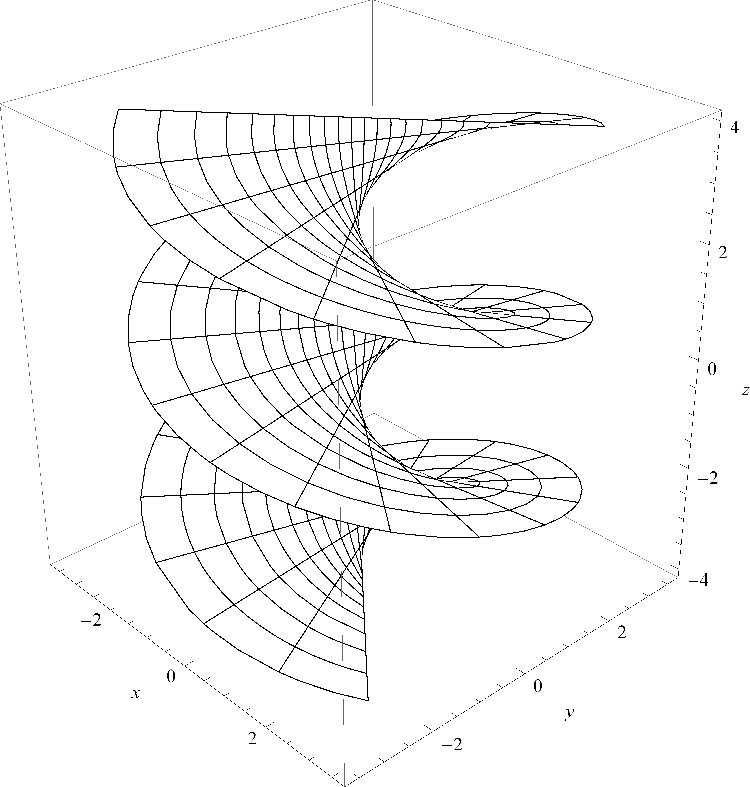
\includegraphics[width=0.5\textwidth]{figures/helicoid.pdf}
      \caption{Helicoid.}
      \label{fig:helicoid}
    \end{figure}
  \end{ex}

  \newcommand{\zint}[2]{\Re#1\int\!#2\,dz}
  % TODO: Catenoid.
  \begin{ex}
    \label{ex:catenoid}
    Let $f = -\frac{e^{-z}}{2}$ and $g = -e^z$, then by the first Weierstrass-Enneper representation, we have
    \begin{multicols}{2}
      \begin{align*}
        x^1 &= \zint{}{-\frac{e^{-z}}{2}\left(1 - e^{2z}\right)}\\
        &= \zint{}{\frac{-e^{-z} + e^z}{2}}\\
        &= \zint{}{\sinh z}\\
        &= \Re\cosh z\\
        &= \cosh u \cos v
      \end{align*}\break
      \begin{align*}
        x^2 &= \zint{}{i\cdot-\frac{e^{-z}}{2}\left(1 + e^{2z}\right)}\\
        &= -\zint{i}{\frac{e^{-z} + e^z}{2}}\\
        &= -\zint{i}{\cosh z}\\
        &= -\Re i\sinh z\\
        &= \Im \sinh z\\
        &= \cosh u \sin v
      \end{align*}
    \end{multicols}
    \begin{align*}
      x^3 &= \zint{2}{-\frac{e^{-z}}{2}\cdot -e^{2z}}\\
      &= \zint{2}{\frac{1}{2}}\\
      &= \Re z\\
      &= u.
    \end{align*}

    This gives us $\bx(u, v) = (\cosh u \cos v, \cosh u \sin v, u)$, which is a catenoid as illustrated in Figure~\ref{fig:catenoid}.
    \begin{figure} % fig: Catenoid
      \centering
      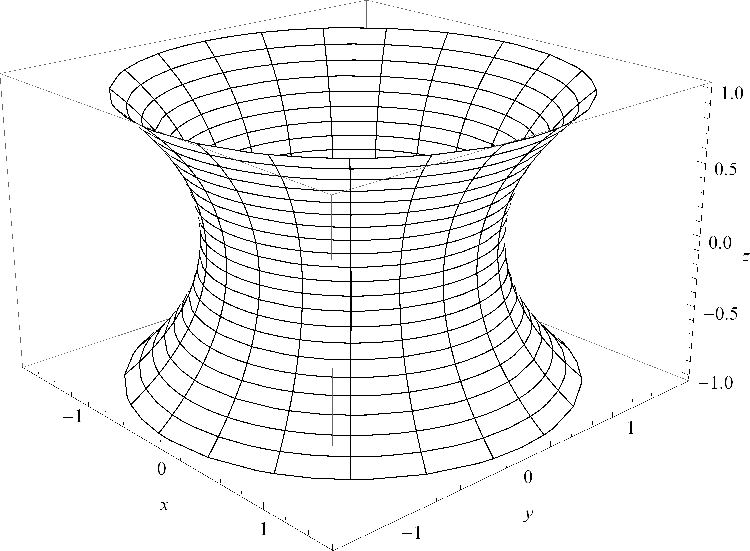
\includegraphics[width=0.5\textwidth]{figures/catenoid.pdf}
      \caption{Catenoid.}
      \label{fig:catenoid}
    \end{figure}
  \end{ex}

  % TODO: Another example.
  \begin{ex}
    Given $F(\tau) = 1$, the surface generated is Enneper's surface, as in Example~\ref{ex:ennepers_surface}. Given that $\tau^3 = \left(f^3 - 3uv^2\right) + i\left(3u^2v - v^3\right)$, observe
    \begin{multicols}{2}
      \begin{align*}
        x^1 &= \tauint{}{(1 - \tau^2)}\\
        &= \tauint{}{1} - \tauint{}{\tau^2}\\
        &= \Re \tau - \frac{1}{3}\Re\tau^3\\
        &= u - \frac{u^3}{3} + uv^2
      \end{align*}\break
      \begin{align*}
        x^2 &= \tauint{}{i(1 + \tau^2)}\\
        &= \tauint{i}{1} + \tauint{i}{\tau^2}\\
        &= \Re i\tau + \frac{1}{3}\Re i\tau^3\\
        &= -\Im\tau - \frac{1}{3}\Im \tau^3\\
        &= - v + \frac{v^3}{3} - vu^2
      \end{align*}
    \end{multicols}
    
    \begin{align*}
      x^3 &= \tauint{2}{\tau}\\
      &= \Re \tau^2\\
      &= (u^2 - v^2).
    \end{align*}
    And we obtain (though with the second coordinate function negated), the standard parameterization of Enneper's surface.
  \end{ex}
}
\pagebreak

%%%%%%%%%%%%%%
%% Bib Data %%
%%%%%%%%%%%%%%

\pagebreak  % This pagebreak is to occur RIGHT BEFORE the bib call-up.  Do not disturb.

\addcontentsline{toc}{section}{References}

% De-comment the next two lines when ready to compile the bibliography.  Use amsplain style.

%\bibliographystyle{amsplain}
%\bibliography{my bib database filename without the .bib extension}

% De-comment the next line to call up the entire database, whether cited or not.
%\nocite*

\end{document}
